%!TEX root = ../main.tex



\section{Εισαγωγή στο LabVIEW}

%\begin{figure}
%  \centering
%  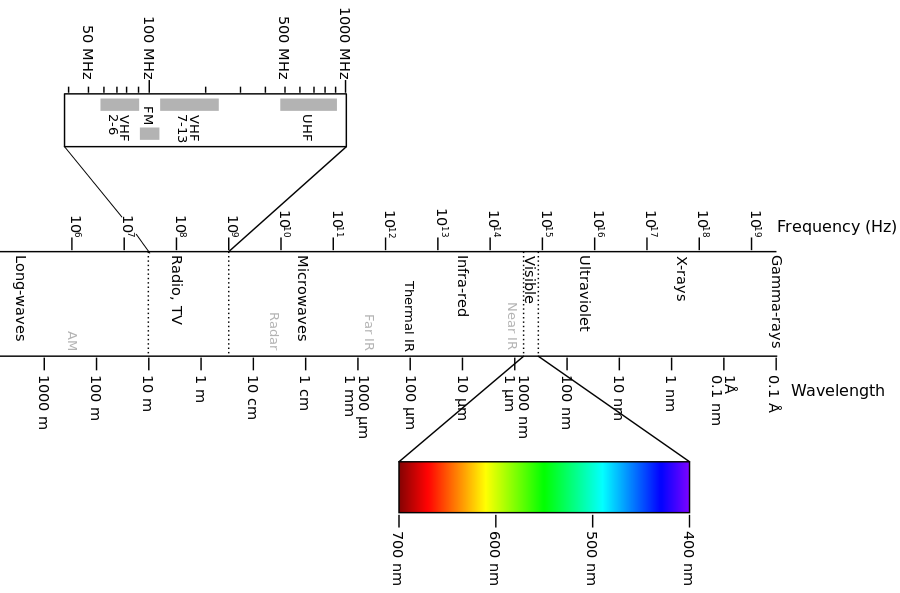
\includegraphics[width=\textwidth]{spectrum}
%  \caption{Το φάσμα της Ηλεκτρομαγνητικής Ακτινοβολίας}
%  \label{fig:spectrum}
%\end{figure}



\lettrine[findent=2pt]{\fbox{\textbf{Τ}}}{ο} λογισμικό που χρησιμοποιήθηκε για την υλοποίηση αυτής της εργασίας είναι το LabVIEW από την εταιρία National Instruments (ΝΙ). Συνεπώς κρίνεται χρήσιμη μια σύντομη αναφορά σε αυτό και στον τρόπο που λειτουργεί. Καθώς το LabVIEW είναι ένα πολύ διαδεδομένο λογισμικό, με ευρεία χρήση στους κλάδους των μηχανικών, κάποιος που θέλει περισσότερες πληροφορίες μπορεί να τις βρει εύκολα στο διαδίκτυο. Κάποιες πηγές που χρησιμοποιήθηκαν για τη συγγραφή αυτής της εργασίας είναι \cite{labview1}, \cite{labview2} και \cite{labview3}. Το LabVIEW (\emph{Laboratory Virtual Instrument Engineering Workbench}) είναι ένα περιβάλλον ανάπτυξης για μία οπτική γλώσσα προγραμματισμού. Σε αντίθεση με τα κοινά προγραμματιστικά περιβάλλοντα, στο LabVIEW δε χρησιμοποιείται κώδικας για να γραφτούν οι εντολές που θα εκτελεστούν αλλά γραφικά όπως κουτιά και σύμβολα. Για παράδειγμα, υπάρχουν πολλές οπτικές γλώσσες, που είναι γνωστές σαν γλώσσες ροής δεδομένων (dataflow), που βασίζονται στην ιδέα "τετράγωνα και βέλη" ("boxes and arrows"), όπου τα τετράγωνα (ή άλλου τύπου αντικείμενα) της οθόνης θεωρούνται οντότητες που συνδέονται από βέλη, γραμμές ή ακμές, που αναπαριστούν σχέσεις μεταξύ τους.

\paragraph{\fbox{\emph{Dataflow Programming}}}Η οπτική γλώσσα προγραμματισμού του LabVIEW ονομάζεται ``G" και βασίζεται στη λογική του \emph{dataflow προγραμματισμού} που αναφέρθηκε προηγουμένως. Αυτό σημαίνει ότι αν υπάρχουν αρκετά δεδομένα διαθέσιμα σε μία συνάρτηση ή ένα subVI (σύνολο συναρτήσεων) τότε αυτή η συνάρτηση ή το subVI θα εκτελεστεί. Η ροή της εκτέλεσης του προγράμματος καθορίζεται από τη δομή ενός γραφικού μπλοκ διαγράμματος (\emph{block diagram}), που στην ουσία αποτελεί τον πηγαίο κώδικα του LabVIEW. Σε αυτό ο προγραμματιστής συνδέει διαφορετικές συναρτήσεις-κόμβους (function-nodes) τραβώντας καλώδια. Αυτά τα καλώδια διαδίδουν τις μεταβλητές και κάθε κόμβος μπορεί να εκτελεστεί μόλις όλα τα δεδομένα στην είσοδό του είναι διαθέσιμα. Δεδομένου ότι αυτό μπορεί να συμβαίνει για πολλαπλούς κόμβους ταυτόχρονα, το LabVIEW μπορεί να εκτελεστεί εγγενώς παράλληλα. Περισσότερα για το dataflow programming μπορείτε να βρείτε στο \cite{dataflow_programming}.

\paragraph{\fbox{\emph{Graphical Programming}}}Το LabVIEW ενσωματώνει τη δημιουργία διεπαφών χρήστη, που ονομάζονται εμπρόσθιοι πίνακες (\emph{front panels}) στον κύκλο ανάπτυξης. Τα προγράμματα-υπορουτίνες LabVIEW ονομάζονται εικονικά όργανα (\emph{VIs}). Κάθε VI διαθέτει τρία στοιχεία: ένα block diagram, ένα front panel και ένα πάνελ σύνδεσης (\emph{connection panel}). Το τελευταίο χρησιμοποιείται για να αντιπροσωπεύει το VI στα block diagrams άλλων, καλώντας τα VI. Το front panel κατασκευάζεται με χειριστήρια (\emph{controls}) και δείκτες (\emph{indicators}). Τα controls είναι είσοδοι: επιτρέπουν σε ένα χρήστη να παρέχει πληροφορίες στο VI. Τα indicators είναι έξοδοι: υποδηλώνουν ή εμφανίζουν τα αποτελέσματα με βάση τις εισόδους που δίδονται στο VI. Το πίσω πλαίσιο, το οποίο είναι ένα block diagram, περιέχει τον γραφικό πηγαίο κώδικα. Όλα τα αντικείμενα που τοποθετούνται στο front panel εμφανίζονται στην πίσω πλευρά ως τερματικά (\emph{terminals}). Ο πίσω πίνακας περιέχει επίσης δομές και λειτουργίες οι οποίες εκτελούν εργασίες στα controls και παρέχουν δεδομένα στα indicators. Οι δομές και οι λειτουργίες βρίσκονται στην παλέτα λειτουργιών και μπορούν να τοποθετηθούν στον πίσω πίνακα. Οι συλλογικοί έλεγχοι, οι δείκτες, οι δομές και οι λειτουργίες θα αναφέρονται ως κόμβοι. Οι κόμβοι συνδέονται μεταξύ τους με τη χρήση καλωδίων, π.χ. δύο controls και μια ενδεικτική λυχνία μπορούν να συνδεθούν με τη λειτουργία προσθήκης (\emph{addition function}) έτσι ώστε η ένδειξη να εμφανίζει το άθροισμα των δύο controls. Έτσι, ένα VI μπορεί να λειτουργήσει είτε ως πρόγραμμα, με τον μπροστινό πίνακα να λειτουργεί ως διεπαφή χρήστη, είτε, όταν πέσει ως κόμβος στο block diagram, το front panel ορίζει τις εισόδους και εξόδους του κόμβου μέσω του παραθύρου σύνδεσης. Αυτό σημαίνει ότι κάθε VI μπορεί εύκολα να δοκιμαστεί πριν να ενσωματωθεί ως υπορουτίνα σε ένα μεγαλύτερο πρόγραμμα.

Η γραφική προσέγγιση επιτρέπει επίσης στους μη προγραμματιστές να χτίσουν προγράμματα με μεταφορά και απόθεση εικονικών αναπαραστάσεων του εργαστηριακού εξοπλισμού με τον οποίο είναι ήδη εξοικειωμένοι. Το περιβάλλον προγραμματισμού LabVIEW, με τα παραδείγματα και την τεκμηρίωση που περιλαμβάνονται, καθιστά απλή τη δημιουργία μικρών εφαρμογών. Αυτό είναι ένα πλεονέκτημα από τη μια πλευρά, αλλά υπάρχει επίσης ο κίνδυνος να υποτιμηθεί η εμπειρογνωμοσύνη που απαιτείται για τον προγραμματισμό G υψηλής ποιότητας. Για σύνθετους αλγορίθμους ή κώδικα μεγάλης κλίμακας, είναι σημαντικό ο προγραμματιστής να έχει εκτεταμένη γνώση της σύνταξης του LabVIEW και της τοπολογίας της διαχείρισης μνήμης της. Τα πιο εξελιγμένα συστήματα ανάπτυξης LabVIEW προσφέρουν τη δυνατότητα δημιουργίας αυτόνομων εφαρμογών. Επιπλέον, είναι δυνατή η δημιουργία κατανεμημένων εφαρμογών, οι οποίες επικοινωνούν με ένα μοντέλο πελάτη-εξυπηρετητή και έτσι είναι ευκολότερο να εφαρμοστούν λόγω της εγγενώς παράλληλης φύσης της προγραμματιστικής γλώσσας G. Ένα τυπικό περιβάλλον προγραμματισμού στο LabVIEW φαίνεται στο σχήμα \ref{fig:labview_example}

\begin{figure}[h]
  \centering
  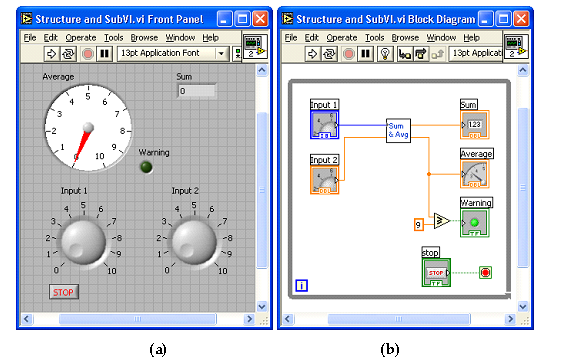
\includegraphics[width=\textwidth]{labview_example}
  \caption{LabVIEW: Front Panel και Block Diagram}
  \label{fig:labview_example}
\end{figure}

%\lettrine[findent=2pt]{\fbox{\textbf{Ό}}}{πως} γνωρίζουμε από την επιστήμη της Φυσικής, όταν ένα σώμα ζεσταθεί αρκετά (π.χ. > 100 \degree C) αρχίζει και εκπέμπει ακτινοβολία και στο οπτικό φάσμα (πέραν του υπέρυθρου), ενώ αποκτά ταυτόχρονα μια ερυθρή όψη. Κατά το φαινόμενο αυτό, η ακτινοβολια που εκπέμπεται ανήκει τόσο στο υπέρυθρο, όσο και στο ορατό φάσμα της ηλεκτρομαγνητικής ακτινοβολίας και μάλιστα το χρώμα που αποκτά το σώμα συνδέεται άμεσα με τη θερμοκρασία στην οποία βρίσκεται. Οι περιοχές της υπέρυθρης και ορατής ακτινοβολίας, καταλαμβάνουν τις ζώνες $1mm - 700nm$ και $700nm - 390nm$ αντίστοιχα, όπως φαίνεται και στο σχήμα \ref{fig:spectrum}.

